\documentclass{article}
\usepackage[margin=1in]{geometry}
\usepackage{amsmath,amsthm,amssymb}
\usepackage{bbm,enumerate,mathtools}
\usepackage{tikz,pgfplots}
\usepackage{chessboard}
\usepackage[hidelinks]{hyperref}
\usepackage{multicol} % Problem 35

\newenvironment{question}{\begin{trivlist}\item[\textbf{Question.}]}{\end{trivlist}}
\newenvironment{note}{\begin{trivlist}\item[\textbf{Note.}]}{\end{trivlist}}
\newenvironment{references}{\begin{trivlist}\item[\textbf{References.}]}{\end{trivlist}}
\newenvironment{related}{\begin{trivlist}\item[\textbf{Related.}]\end{trivlist}\begin{enumerate}}{\end{enumerate}}


\begin{document}
\rating{2}{1}
Let a ``polyarc'' be a path composed of quarter circular arcs, and a polyarc-configuration be
a placement of polyarcs on an $n \times m$ grid such that no part of a polyarc is
inside another polyarc.
\begin{figure}[ht!]
  \centering
  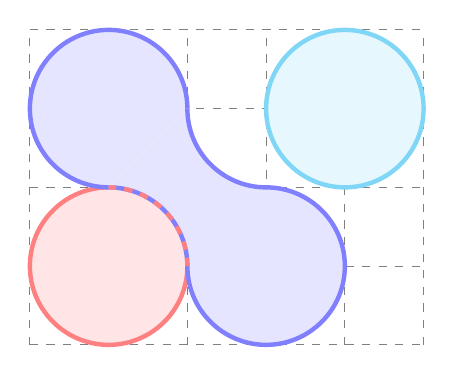
\begin{tikzpicture}
    \draw[gray, dashed] (0, 0) grid (5, 4);
    \fill[ultra thick, blue!10]
      (1,2) arc (90:0:1)--
      (3,2) arc (270:180:1);
    \fill[red!10] (1,1) circle (1);
    \draw[ultra thick, red!50] (1,2) arc (90:360:1);
    \draw[ultra thick, blue!50, fill=blue!10]
      (2,1) arc (180:450:1)
      (2,3) arc (0:270:1);
    \draw[ultra thick, blue!50]
      (1,2) arc (90:0:1)
      (3,2) arc (270:180:1);
    \draw[ultra thick, red!50, dashed]        (2,1) arc (0:90:1);
    \draw[ultra thick, cyan!50, fill=cyan!10] (5,3) arc (0:360:1);
  \end{tikzpicture}
  \caption{
    An example of a polyarc-configuration
  }
\end{figure}
\begin{question}
  How many such polyarc-configurations exist on the $n \times m$ grid?
\end{question}

\begin{related}
  \item What if polyarcs can be inside other polyarcs?
  \item What if all polyarcs must be tangent to another polyarc?
  \item With if the polyarc-configuration must be connected?
  \item What configuration gives maximum area for the entire polyarc-configuration?
  \item Can this be done on a triangular/hexagonal grid with $1/3$ or $1/6$ arcs?
  \item How many different non-self-intersecting $4$-robot walks can fit inside
    of an $n \times m$ grid? Self-intersecting?
  \item What if instead of quarter circles, boxes were made with diagonal line
    segments?
  \item Is there a nice multi-dimensional analog?
\end{related}
\begin{references}
  \item Problem 79.
\end{references}
\end{document}
